\section{System Description}
The challenge as described was clearly separated into two phases. First, we needed to classify the given audio samples into normal or pathological. Then, the pathological samples were to be classified into one of three kinds: vocal palsy, phonotrauma or neoplasm. Upon an initial inspection and analysis of the data, we observed that vocal palsy seemed the easiest to tell apart from normal by listening to the samples. Therefore, we decided upon a pipeline based approach (Figure~\ref{fig:}). In the pipeline, after preprocessing, we first check if a new sample is normal or not. If a sample is classified as abnormal, it is sent to the second stage, where we decide if it is a sample corresponding to vocal palsy. If this stage returns negative, we proceed to the final stage where the sample is assigned a label corresponding to either phonotrauma or neoplasm. An advantage of this approach instead of a simple multiclass approach is that, by eliminating many samples for consideration by the later stages of the pipeline, we may hope to improve accuracy over classifying everything at once. On the other hand, this approach leaves the most ``confusing" examples for the last classifier, and since we do not have the option of returning an ``I don't know" label, it may be that our phonotrauma vs neoplasm classifier could have a lower accuracy.

The next consideration was the algorithm to use as a classifier in each stage. Recent machine learning systems and competitions have shown that ensemble approaches are often the best at solving complex problems. This is because typically, a diverse ensemble of classifiers can have elements that each focus on a different aspect of the problem so that when results are combined, the entire system does well. We also chose to follow this principle in designing our classifiers. 

The next question to answer was how to design our ensemble. Rather than going with an off-the-shelp approach, we chose to build an ensemble to 

Recent challenges in machine learning indicate that many tasks can be best handled with an ensemble approach. 
\subsection{Data Preprocessing and Implementation Details}
	Doing a spot check on both training and testing set, we discovered that there exists silence or noise at the beginning of most audio files. We removed those silence or noise parts by calculating the average loudness of each audio file, and recursively comparing the value of 30\% of average loudness to first $\frac{3}{4}$ of the audio file.

\subsection{Validation Method:}
Before mentioning detailed structure and algorithm we have attempted, I want to point out that we measure accuracy using stratified 10-fold cross validation(CV). Any classifier's accuracy is the weighted average accuracy of numbers we get from 10 folds.  \\
\indent However, for transductive learning algorithm such as Transductive Support Vector Machine or Label Propagation, we could not do cross validation since there is no validation set for transductive learning. Accuracy we have on those algorithms is the accuracy on whole training set, in other word, the rate of convergence. 
% % \subsection{Attempted Algorithms:}
% Tree-Based Algorithms:
% \begin{itemize}
	% \item Decision Tree:\\
	% Utilizing tree structures, decision tree algorithm calculates entropy of each feature and splits node based on the rank of features with respect to their entropies. Probably due to the fact that different classes are representative in different features and skewed class distribution, a single decision tree could not solve this learning problem and we only get 62\% accuracy on CV.\\
	% \item Random Forest:\\
	% Instead of having a single tree structure, Random Forest fits a number of decision tree classifiers on various sub-samples of the dataset.\cite{b7} Using Random Forest classifier, we get 89\% accuracy on CV. But even with such high accuracy, Random Forest performs poorly on test set according to the feedback from oracle. We analyze that the differences on performance between training set and testing set probably result from skewed data distribution and over-fitting. \\
% \end{itemize}

% \indent Based on cross validation results on experiments we have done, it seems like tree-based algorithm generally is inappropriate for this learning task. \\

Support Vector Machines(SVMs):\\
\begin{itemize}
	\item Linear SVM:\\
	Based on the features' distribution of each training example, SVM differentiates classes by building a hyperplane that maximizes the margin between classes. And for Linear SVM, the decision boundary is a linear function. The kernel of Linear SVM is simply the hyperplane function $K(x_i,x_j) = \phi(x_i)*\phi(x_j) = (x_i*x_j)^2$, and in order to maximize the margin between plus-plane and minus-plane to get best generalization, SVM minimized the norm of parameter $w$\cite{b12}. After tuning loss penalty and class weight, we get 89\% accuracy on CV and a relatively reasonable classification on test set according to the feedback from oracle.\\
	\item SVM with Radial Basis Function kernel(SVM-RBF):\\
	Pretty similar to Linear SVM, SVM-RBF differs by the non-linear kernel function. The SVM-RBF formulation differs from Linear SVM by having an non-linear kernel function, which could be represented as $K(x_i,x_j) = exp(-\gamma||x_i - x_j ||^2)$\cite{b12}. After having a reasonable result from Linear SVM, we were excited on trying SVM-RBF(with tuned loss penalty and gamma). It ends up having 89\% on CV and similar test set performance. However in the late phase, we discarded SVM-RBF because with the number of features we have, it is possible that a non-linear kernel function over-fits. \\
\end{itemize}

Transductive Learning Algorithms:\newline\\
\indent Noticing that size of test set is twice size of training set, in order to get better generalization, we want to utilize test set and attempted several transductive learning algorithms. \\
\begin{itemize}
	\item Label Propagation:\\
	Identifying the test example's closest training set neighbor, Label Propagation assigns the same label that neighbor has to the test example. The edge between any two examples i and j, is weighted to be so that the closer the nodes are in local Euclidean distance, the larger the weight $w_{ij}$, the weight is controlled by a parameter $\theta$ :  $w_{ij} = exp (\frac{(d_{ij}^2)}{\theta^2}) = exp (-\frac{\sum_{d = 1}^{D} (x_{id} - x_{jd})^2}{\theta^2} )$. \cite{b13}Without CV on this algorithm, we compare the number of assigned labels of each class to that from SVMs. From Label Propagation, we get 69 Normals, 107 Vocal Palsys and 171 Phonotraumas. From Linear SVM, we get 65 Normals, 79 Vocal Palsys and 167 Phonotraumas.\\
	\item Transductive Support Vector Machine(TSVM):\\
	This is a SVM-RBF based classifier with test set regulating the range of how far away the hyperplane can extends. The kernel function of SVM-RBF is represented as $K(x_i,x_j) = exp(-\frac{||x_i - x_j ||^2}{2\gamma^2})$\cite{b14}. Although in test set, TSVM overcalls a great number of Normal, it could give us a board view of all 'Normal-ish' examples, and later on we could limit our focus on this specific set of Normals. \\
\end{itemize}

Multiple Instance Learning Regression(MILR):\\
\begin{itemize}
	\item 
	Instead of receiving a set of instances which are individually labeled, the learner receives a set of labeled bags, each containing many instances. In the simple case of multiple-instance binary classification, a bag may be labeled negative if all the instances in it are negative. On the other hand, a bag is labeled positive if there is at least one instance in it which is positive. \cite{b10} Although MILR undercalls Normal, having super high Area under ROC Curve(AUC) 0.92, MILR could work as an oracle and we only focus on test examples labeled with confidence higher than 85\%.\\
\end{itemize}
\subsection{Final Architecture Overview:}
	Our whole model-building infrastructure is based on scikit-learn\cite{b7}\cite{b8}. \\
	\indent We tried Support Vector Machine, Boosting, Random Forest, Extratrees, Multiple Instance Learning, Label Propagation. After few experiments, it seemed like tree algorithms performed poorly on this task and we finalized our focus on SVM, Label Propagation, SVM-RBF and MILR with pipeline. Any single classifier undercalled Normal and Neoplasm patients, which we think is resulted from different class distributions between training and testing set. \\
\indent So, we converted this relatively complex learning task into three less complicated tasks: Normal vs. Pathological, Vocal vs. Rest of Diseases, and Phonotrauma vs. Neoplasm, with each learning task having ensemble consisted of 4 classifiers.[Fig. 1] The reason why we design the pipeline this way is based on the difficulty of classification according to our perception. (From easiest Normal vs. Pathological to hardest Phonotrauma vs. Neoplasm)\\
	\begin{figure}[!htbp]
		\begin{center}
			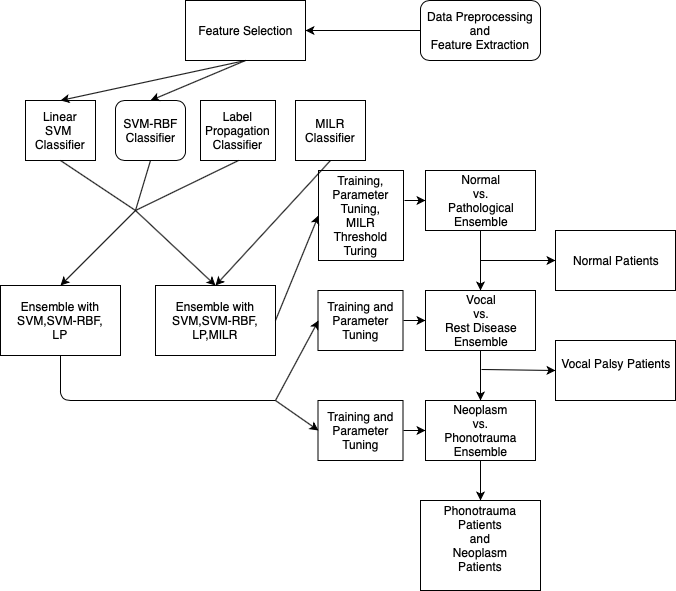
\includegraphics[scale=0.35]{Diagram_3.png}
		\end{center}
		\caption{The Process of Classifying, including classifier training, ensemble structures and pipeline implementation}
	\end{figure}

\subsection{Feature Selection:}
Due to the fact that the size of our training set is relatively small, in case of over-fitting, for each classifier we select 50\% best features, with respect to entropy, according to Renyi's feature selection.\cite{b14} However, it seems like feature selection jeopardizes the performance of transductive learning. So we only utilize feature selection on SVM and SVM-RBF.

\subsection{Hyper Parameter Tuning:}
Since the size of training set is getting smaller and smaller as we propagate through the pipeline, in order to get trustworthy accuracy to tune parameter for SVC, for all three ensembles, we use the same parameter tuned in the first ensemble. The process is pretty straightforward; we simply set up two loops, one of which for C and one of which for gamma. The tuned parameters are 10 for C, and 0.01 for gamma. Also due to the skewed distribution in training set, we modify the class weight with respect to the proportion of class. 


